%%%%%%%%%%%%%%%%%%%%%%%%%%%%%%%%%%%%%%%%%%%%%%%%%%%%%%%%%%%%%%%%
%%                                                            %%
%% aGreekPrimer, Italian translation 2016.12 - 2017           %%
%%                                                            %%
%% From:  Clarence W. Gleason, A Greek Primer                 %%
%%        (1903, New York, American Book Company)             %%
%%                                                            %%
%%        https://archive.org/details/greekprimer00glea       %%
%%                                                            %%
%% Translated by g.p.ciceri <gp.ciceri@gmail.com>             %%
%% ---------------------------------------------------------- %%
%% This translation is Licensed under                         %%
%% Creative Commons Attribution-ShareAlike 4.0 International  %%
%% https://creativecommons.org/licenses/by-sa/4.0/            %%
%%                                                            %%
%%%%%%%%%%%%%%%%%%%%%%%%%%%%%%%%%%%%%%%%%%%%%%%%%%%%%%%%%%%%%%%%

% ᾶῖῶῆῦ  
% ἀἰὐἐὀὠἠ 
% ὰὲὶὸὺὼὴ 
% ἁἱὑὁὡἡῥ
% άέίόύήώΆΉ
% ἂἒὒἲὂὢἢὒἚἊ
% ἃἳὓὃἣὣἓἋἛ
% ἄἔἴὄὔὤἤἌἬ
% ἅἕἵὅὕὥἥἍἭ
% ἆὦἶἦὖἯἏὯἇὧἷἧὗἯἏὯ 

% ᾳῃῳ
% ᾱῑῡ
% ᾀᾐᾠ
% ᾰῐῠ
% ᾂᾒᾢ
% ϊ ϋ
% ᾄᾔᾤ
% ΰ ΐ
% ᾆᾖᾦ
% ᾲῂῲ
% ᾴῄῴ
% ᾷῇῷ
% ᾳῃῳ
% ᾱῑῡ
% ᾰῐῠ

% āēīōū
% ăĕĭŏŭ

% ᾳῃῳ
% ᾷῇῷ


\documentclass[nols]{tufte-handout}

%\geometry{showframe} % display margins for debugging page layout

\usepackage{fontspec}
\usepackage{ifxetex}
\setmainfont[Path=./fonts/palatino-linotype/, ItalicFont=palai.ttf, BoldFont=palab.ttf]{pala.ttf}
%\setmainfont[Path=./fonts/GFS_Didot/, ItalicFont=GFSDidotItalic.ttf, BoldFont=GFSDidotBold.ttf]{GFSDidot.ttf}

\newfontfamily\GFSDidotBf[Path=./fonts/GFS_Didot/]{GFSDidotBold.ttf}
\newfontfamily\GFSDidot[Path=./fonts/GFS_Didot/]{GFSDidot.ttf}

\newcommand{\didobf}[1]{{\GFSDidotBf #1}}
\newcommand{\dido}[1]{{\GFSDidot #1}}


\usepackage{lipsum}
\usepackage{url}
\usepackage{longtable}
\usepackage{stackengine}

\usepackage{graphicx} % allow embedded images
  \setkeys{Gin}{width=\linewidth,totalheight=\textheight,keepaspectratio}
  \graphicspath{{graphics/}} % set of paths to search for images
\usepackage{amsmath}  % extended mathematics
\usepackage{booktabs} % book-quality tables
\usepackage{units}    % non-stacked fractions and better unit spacing
\usepackage{multicol} % multiple column layout facilities
\usepackage{lipsum}   % filler text
\usepackage{fancyvrb} % extended verbatim environments
  \fvset{fontsize=\normalsize}% default font size for fancy-verbatim environments

% Standardize command font styles and environments
\newcommand{\doccmd}[1]{\texttt{\textbackslash#1}}% command name -- adds backslash automatically
\newcommand{\docopt}[1]{\ensuremath{\langle}\textrm{\textit{#1}}\ensuremath{\rangle}}% optional command argument
\newcommand{\docarg}[1]{\textrm{\textit{#1}}}% (required) command argument
\newcommand{\docenv}[1]{\textsf{#1}}% environment name
\newcommand{\docpkg}[1]{\texttt{#1}}% package name
\newcommand{\doccls}[1]{\texttt{#1}}% document class name
\newcommand{\docclsopt}[1]{\texttt{#1}}% document class option name
\newenvironment{docspec}{\begin{quote}\noindent}{\end{quote}}% command specification environment

% concetti morfosintattici
\usepackage{xspace} 
\newcommand{\noun}{\textsc{sostantivo}\xspace}
\newcommand{\nouns}{\textsc{sostantivi}\xspace}
\newcommand{\adject}{\textsc{aggettivo}\xspace}
\newcommand{\adjects}{\textsc{aggettivi}\xspace}
\newcommand{\gnumber}{\textsc{numero}\xspace}
\newcommand{\gnumbers}{\textsc{numeri}\xspace}
\newcommand{\gender}{\textsc{genere}\xspace}
\newcommand{\genders}{\textsc{generi}\xspace}
\newcommand{\gcase}{\textsc{caso}\xspace}
\newcommand{\gcases}{\textsc{casi}\xspace}
\newcommand{\tense}{\textsc{tempo}\xspace}
\newcommand{\mood}{\textsc{modo}\xspace}
\newcommand{\gverb}{\textsc{verbo}\xspace}
\newcommand{\gverbs}{\textsc{verbi}\xspace}
\newcommand{\adjective}{\textsc{aggettivo}\xspace}
\newcommand{\nom}{\textsc{nom}\xspace}
\newcommand{\gen}{\textsc{gen}\xspace}
\newcommand{\dat}{\textsc{dat}\xspace}
\newcommand{\acc}{\textsc{acc}\xspace}
\newcommand{\voc}{\textsc{voc}\xspace}
\newcommand{\gexit}{\textsc{uscita}\xspace}
\newcommand{\gexits}{\textsc{uscite}\xspace}
\newcommand{\declinazione}{\textsc{declinazione}\xspace}
\newcommand{\masc}{\textsc{maschile}\xspace}
\newcommand{\femm}{\textsc{femminile}\xspace}
\newcommand{\neut}{\textsc{neutro}\xspace}

\newcommand{\indic}{\textsc{indicativo}\xspace}
\newcommand{\imper}{\textsc{imperativo}\xspace}
\newcommand{\gcong}{\textsc{congiuntivo}\xspace}
\newcommand{\ott}{\textsc{ottativo}\xspace}
\newcommand{\partic}{\textsc{participio}\xspace}
\newcommand{\infin}{\textsc{infinito}\xspace}

\newcommand{\pres}{\textsc{presente}\xspace}
\newcommand{\imperf}{\textsc{imperfetto}\xspace}
\newcommand{\aor}{\textsc{aoristo}\xspace}
\newcommand{\fut}{\textsc{futuro}\xspace}
\newcommand{\perf}{\textsc{perfetto}\xspace}
\newcommand{\pperf}{\textsc{piuccheperfetto}\xspace}

\newcommand{\sing}{\textsc{singolare}\xspace}
\newcommand{\plur}{\textsc{plurale}\xspace}
\newcommand{\dual}{\textsc{duale}\xspace}

\newcommand{\si}{\textsc{sing}\xspace}
\newcommand{\pl}{\textsc{plur}\xspace}
\newcommand{\du}{\textsc{dual}\xspace}

\newcommand{\att}{\textsc{attivo}\xspace}
\newcommand{\med}{\textsc{medio}\xspace}
\newcommand{\pass}{\textsc{passivo}\xspace}
\newcommand{\medpass}{\textsc{medio-passivo}\xspace}


% italianitudini
\renewcommand{\figurename}{Figura}
\renewcommand{\tablename}{Tabella}
\renewcommand{\contentsname}{Indice}

% fix per un qualche problema
\ifxetex
  \newcommand{\textls}[2][5]{%
    \begingroup\addfontfeatures{LetterSpace=#1}#2\endgroup
  }
  \renewcommand{\allcapsspacing}[1]{\textls[15]{#1}}
  \renewcommand{\smallcapsspacing}[1]{\textls[10]{#1}}
  \renewcommand{\allcaps}[1]{\textls[15]{\MakeTextUppercase{#1}}}
  \renewcommand{\smallcaps}[1]{\smallcapsspacing{\scshape\MakeTextLowercase{#1}}}
  \renewcommand{\textsc}[1]{\smallcapsspacing{\textsmallcaps{#1}}}
\fi

% too many float...
\extrafloats{100}

\title{A Greek Primer. Introduzione al Greco Antico \newline Lezione XV - Temi in Linguale della Declinazione in Consonante.}

\author[gpciceri]{a cura di Milagathòs: Milo's help to enjoy humanities}

\date{17 Gennajo 2017} % without \date command, current date is supplied


\begin{document}

\maketitle% this prints the handout title, author, and date

\begin{marginfigure}[-2.0cm]
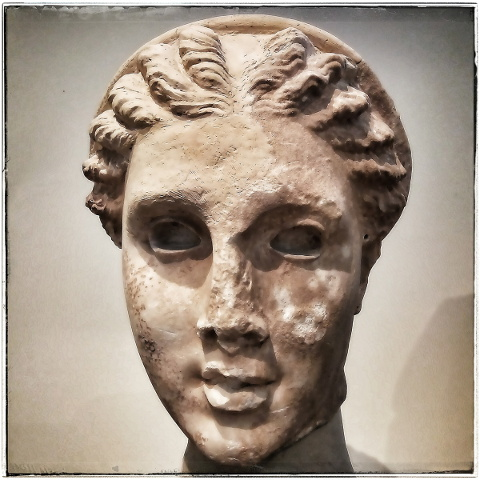
\includegraphics{smallthumb-lesson_XIII.jpeg}
\setfloatalignment{b}
\end{marginfigure}


\begin{abstract}
\noindent
Queste lezioni si articolano in \textsc{elementi grammaticali}, 
espressi sommariamente, seguiti da \textsc{vocabolari} per il lessico di base 
e da \textsc{frasi da tradurre} dal greco e in greco. 
\
L'approccio è quello del testo-laboratorio di morfosintassi: 
si presenta punto per punto - riprendendone la numerazione - 
l'esposizione di Gleason\cite{gleason1903}.\\
\bigskip
\noindent
Lezione XV: temi in Linguale della Declinazione in Consonante; vocabolario, esercizi.
\end{abstract}

%\printclassoptions

\newthought{166.} Nella maggior parte dei temi in linguale (\didobf{τ, δ, θ}), 
questa cade davanti alla \didobf{ς} per formare il nominativo singolare, come in \didobf{ἐλπιδ-}, \textit{la speranza} \nom \didobf{ἐλπίς} e in \didobf{ὀρνιθ-}, \textit{l'uccello} \nom \didobf{ὄρνις}; ma nei nomi il cui tema termina in \didobf{-οντ}, la \didobf{τ} cade e la \didobf{ο} si allunga a \didobf{ω}, come in \didobf{λεοντ-}, \textit{il leone} \nom \didobf{λέων}.
Nei nomi neutri il nominativo singolare coincide con il tema, una volta caduta da quest'ultimo la \didobf{τ} finale\sidenote{le sole consonanti che possono stare alla fine di una parola sono \didobf{ν, ρ, ς} (\didobf{ψ = πς, ξ = κς.})}; come in \didobf{σωματ-}, \textit{il corpo} \nom \didobf{σῶμα}.


\newthought{162. Modelli}

\begin{fullwidth}
\begin{table}[!htbp]
  \centering
  \begin{tabular}{l l l l l l l l l l l l}
    %\toprule
	\multicolumn{12}{c}{\textsc{III Declinazione - Temi in Linguale}} \\
	
	\multicolumn{2}{c}{\didobf{ὄρνις, ὁ, ἡ,}} 
	& \didobf{ἐλπίς, ἡ,} 
	& \multicolumn{3}{c}{\didobf{οὗτος ὁ λέων,}}
	& \multicolumn{3}{c}{\didobf{τοῦτο τὸ σῶμα,}}
	
	& \hspace{3 mm} & \multicolumn{2}{c}{\textsc{Termin. Neutro.}} \\
	
	\multicolumn{2}{c}{\textit{uccello}}
	& \multicolumn{1}{c}{\textit{speranza}}
	& \multicolumn{2}{r}{\textit{questo}} & \multicolumn{1}{l}{\textit{leone}}
	& \multicolumn{2}{r}{\textit{questo}} & \multicolumn{1}{l}{\textit{corpo}}
	& \hspace{3 mm}
	& \multicolumn{1}{l}{\textsc{Greco}} & \multicolumn{1}{l}{\textsc{Latino}} \\
   
	\multicolumn{12}{c}{\textsc{singolare}} \\
	
    \textsc{n.} & \didobf{ὄρνις}   & \didobf{ἐλπίς}   & \didobf{οὗτος}  & \didobf{ὁ} & \didobf{λέων} & \didobf{τοῦτο}  & \didobf{τὸ} & \didobf{σῶμα}  & \hspace{3 mm} & \textemdash & \textemdash \\
	
    \textsc{g.} & \didobf{ὄρνιθος}   & \didobf{ἐλπίδος}   & \didobf{τούτου}  & \didobf{τοῦ} & \didobf{λέοντος} & \didobf{τούτου}  & \didobf{τοῦ} & \didobf{σώματος}  & \hspace{3 mm} & \didobf{ος} & is \\
	
	\textsc{d.} & \didobf{ὄρνιθι}   & \didobf{ἐλπίδι}   & \didobf{τούτῳ}  & \didobf{τῷ} & \didobf{λέοντι} & \didobf{τούτῳ}  & \didobf{τῷ} & \didobf{σώματι}  & \hspace{3 mm} &  \didobf{ι} & ī \\
	
	\textsc{a.} & \didobf{ὄρνιν}   & \didobf{ἐλπίδα}   & \didobf{τοῦτον}  & \didobf{τὸν} & \didobf{λέντα} & \didobf{τοῦτον}  & \didobf{τὸν} & \didobf{σῶμα}  & \hspace{3 mm} & \textemdash & \textemdash \\
	
	\textsc{v.} & \didobf{ὄρνις}   & \didobf{ἐλπί}   & \textemdash  & \textemdash & \didobf{λέον} & \textemdash  & \textemdash & \didobf{σῶμα}  & \hspace{3 mm} & \textemdash & \textemdash \\
	
	\multicolumn{12}{c}{\textsc{plurale}} \\
	
	
	\textsc{n.} & \didobf{ὄρνιθες}   & \didobf{ἐλπίδες}   & \didobf{οὗτοι}  & \didobf{οἱ} & \didobf{λέοντες} & \didobf{ταῦτα}  & \didobf{τὰ} & \didobf{σώματα}  & \hspace{3 mm} & \didobf{ᾰ} & ă \\
	
    \textsc{g.} & \didobf{ὄρνιθων}   & \didobf{ἐλπίδων}   & \didobf{τούτων}  & \didobf{τῶν} & \didobf{λέοντων} & \didobf{τούτων}  & \didobf{τῶν} & \didobf{σωμάτων}  & \hspace{3 mm} & \didobf{ων} & um \\
	
	\textsc{d.} & \didobf{ὄρνισι}   & \didobf{ἐλπίσι}   & \didobf{τούτοις}  & \didobf{τοῖς} & \didobf{λέουσι} & \didobf{τούτοις}  & \didobf{τοῖς} & \didobf{σώματασι}  & \hspace{3 mm} &  \didobf{σι} & ibus \\
	
	\textsc{a.} & \didobf{ὄρνιθας}   & \didobf{ἐλπίδας}   & \didobf{τούτους}  & \didobf{τοῦς} & \didobf{λέοντας} & \didobf{ταῦτα}  & \didobf{τὰ} & \didobf{σώματα}  & \hspace{3 mm} & \didobf{ᾰ} & ă \\
	
	\textsc{v.} & \didobf{ὄρνιθες}   & \didobf{ἐλπίδες}   & \textemdash  & \textemdash & \didobf{λέοντες} & \textemdash  & \textemdash & \didobf{σώματα}  & \hspace{3 mm} & \didobf{ᾰ} & ă \\
	
	%\bottomrule
  \end{tabular}
  \label{tab:normaltab}
  %\zsavepos{pos:normaltab}
\end{table}
\end{fullwidth}

\newthought{Osservazioni}
\begin{itemize}
\item[\textsc{1.}] Nota come il pronome dimostrativo \didobf{οὗτος} sia usato assieme all'articolo ma che \textbf{non} stia tra l'articolo e il nome, come succede per un aggettivo. Questa posizione viene detta \textit{posizione predicativa}\sidenote{questo è il leone.}. L'articolo non viene tradotto. 
\end{itemize}

\newthought{168. Particolarità dei Temi in Linguale}
\begin{itemize}
\item[\textsc{1.}] Nei linguali con nominativo in \didobf{-ις}, eccetto gli ossitoni, la linguale cade all' \acc \si e viene aggiunta una \didobf{ν}, come in \didobf{ὄρνις} \acc \didobf{ὄρνιν}. 
\item[\textsc{2.}] In tutti i temi in \didobf{-ιδ}, e in quelli in \didobf{-ντ} non ossitoni, il \voc \si è formato dal tema senza la linguale \didobf{δ, τ}, come in \didobf{ἐλπίς} \voc \didobf{ἐλπί}.
\item[\textsc{3.}] Le consonanti \didobf{ντ, νδ, νθ} (\didobf{ν} seguita da linguale) prima di una \didobf{ς} cadono e la vocale che le precede viene allungata (\didobf{ε} diventa \didobf{ει}, \didobf{ο} diventa \didobf{ου}) come in 
\didobf{λέουσι} (da \didobf{λέοντ-σι}).
\end{itemize}

\newthought{(696). Pronome Dimostrativo}

\begin{fullwidth}
\begin{table}[!htbp]
  \centering
  \begin{tabular}{l l l l}
    %\toprule
	\multicolumn{4}{c}{\didobf{οὗτος}, \textsc{questo}} \\
	\multicolumn{4}{c}{\sing} \\
	
	& \masc & \femm & \neut \\
	
	\textsc{n.} & \didobf{οὗτος} & \didobf{αὕτη} & \didobf{τοῦτο} \\
	\textsc{g.} & \didobf{τούτου} & \didobf{ταύτης} & \didobf{τούτου} \\
	\textsc{d.} & \didobf{τούτῳ} & \didobf{ταύτῃ} & \didobf{τούτῳ} \\
	\textsc{a.} & \didobf{τοῦτον} & \didobf{ταύτην} & \didobf{τοῦτο} \\
	
	\multicolumn{4}{c}{\plur} \\
	
	& \masc & \femm & \neut \\
	
	\textsc{n.} & \didobf{οὗτοι} & \didobf{αὗται} & \didobf{ταῦτα} \\
	\textsc{g.} & \didobf{τούτων} & \didobf{τούτων} & \didobf{τούτων} \\
	\textsc{d.} & \didobf{τούτοις} & \didobf{τούταις} & \didobf{τούτοις} \\
	\textsc{a.} & \didobf{τοῦτους} & \didobf{ταύτας} & \didobf{ταῦτα} \\
	
	%\bottomrule
  \end{tabular}
  \label{tab:normaltab}
  %\zsavepos{pos:normaltab}
\end{table}
\end{fullwidth}


\newthought{169. Vocabolario}

\begin{multicols}{2}
    \noindent \hangindent=1em \didobf{ἐλπις, ἐλπίδος, ἡ} \textit{speranza}.  \\
    \noindent \hangindent=1em \didobf{λέων, λέοντος, ὁ} \textit{leone}.  \\
    \noindent \hangindent=1em \didobf{νύξ, νυκτός, ἡ} \textit{notte}.  \\
    \noindent \hangindent=1em \didobf{ὄνομα, ὄνόματος, τό} \textit{nome}.     \\
    \noindent \hangindent=1em \didobf{σῶμα, σώοματος, τό} \textit{corpo}.  \\
    \noindent \hangindent=1em \didobf{φυγάς, φυγατος, ὁ} \textit{esilio}.  \\
    \noindent \hangindent=1em \didobf{φωνή, ἡ} \textit{voce}.  \\
	
    \noindent \hangindent=1em \didobf{οὗτος, αὕτη, τοῦτο} pron.dimostr. \textit{questo (696)}.  \\
	
	\noindent \hangindent=1em \didobf{χαλεπός, ή, όν} agg. \textit{duro, severo, grezzo}.  \\
	
    \noindent \hangindent=1em \didobf{ἥκω}, fut. \didobf{ἥξω}, \textit{venire, essere venuto}.  \\
	
	\noindent \hangindent=1em \didobf{σύν} prep. con \dat \textit{con}.  \\
	
\end{multicols}


\newthought{170. Traduci:}
\textsc{1.}~\dido{ἡμέρας καὶ νύκτας δέκα ἔβαλλον λίθους εἰς τὴν διώρυχα.} \quad
\textsc{2.}~\dido{οἱ γὰρ τῶν φυγάδων υἱοὶ ταχέως ἧκον εἰς τὴν κώμην.} \quad
\textsc{3.}~\dido{καὶ οὗτοι οἱ στρατιῶται ἦσαν ἐν ἐλπίσι καλαῖς τῆς νίκης.} \quad
\textsc{4.}~\dido{ἀλλὰ οὐχ ἱκανοὶ ἦσαν διώκειν τοὺς πολεμίους ἐκ τοῦ χωρίου.} \quad
\textsc{5.}~\dido{οἱ δὲ πολῖται σὺν τοῖς τέκνοις εὐθὺς ἥξουσιν ἐπὶ τὸν ποταμόν.} \quad
\textsc{6.}~\dido{οὗτος ὁ σατράπης ἦν Πέρσης, ὄνομα Ξέρξνς.} \quad
\textsc{7.}~\dido{καὶ τεθηρεύκασι λέοντας οἱ ἐκ τῆς κώμης νεσνίαι.} \quad
\textsc{8.}~\dido{καὶ μετὰ τῶν ὀρνίθων ηὗρον ὀλίγους πέρδικας.} \quad
\textsc{9.}~\dido{μικρὰ γὰρ εἶχον σώματα, ἀλλ´αἱ κεφαλαὶ μακραὶ ἦσαν.} \quad
\textsc{10.}~\dido{ἔρριψε, θαυμάσεις, ἐλελύκης, πίνομεν, κλέπτει, ηὗρε, πεπείκατε.}

\newthought{171. Scrivi in Greco:}
\textsc{1.}~Ma gli uomini erano grezzi nel parlare\sidenote{in che caso? cfr. (148.)}. \quad
\textsc{2.}~Impararono a cacciare a scuola. \quad
\textsc{3.}~Se ha mandato i regali, l'esercito ha la (sua) paga. \quad

\begin{figure}[!b]
  %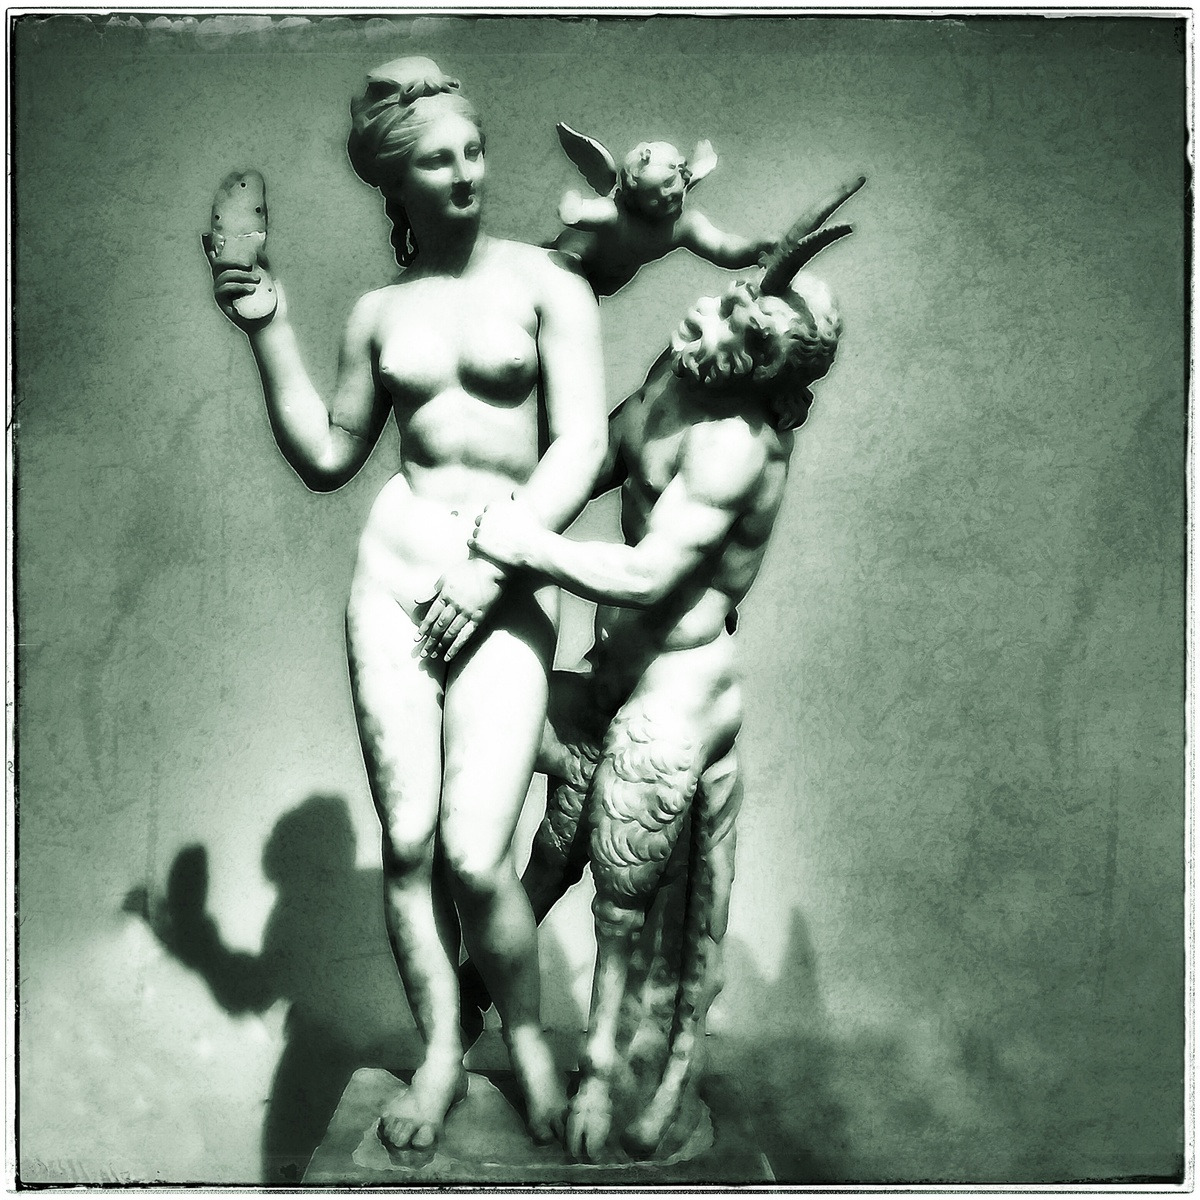
\includegraphics[width=0.8\linewidth]{thumb-lesson_XV.jpeg}
  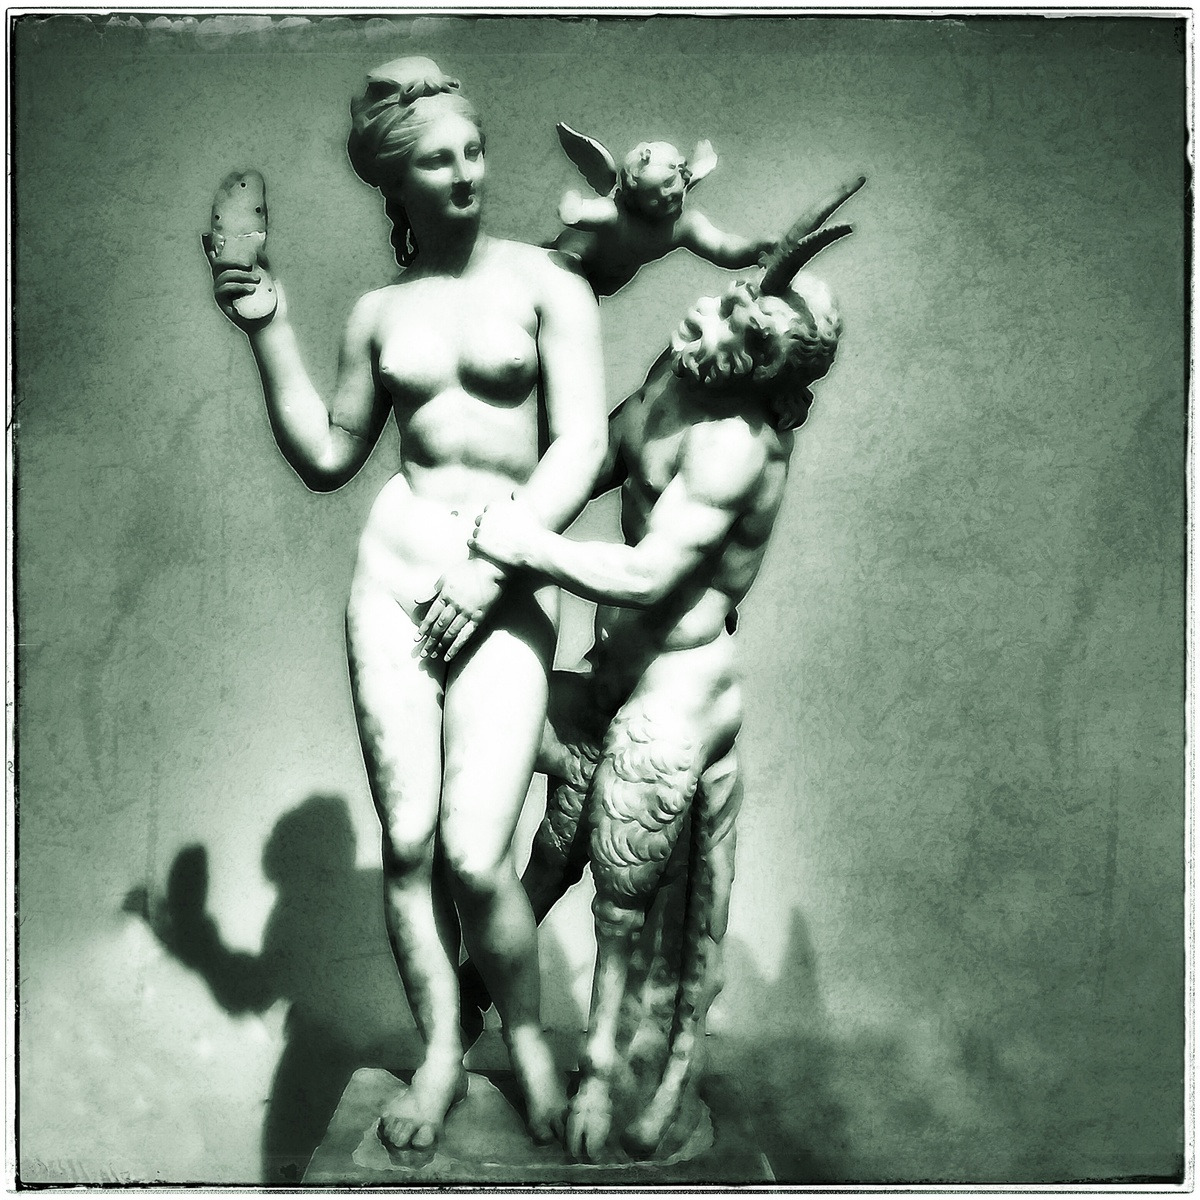
\includegraphics{thumb-lesson_XV.jpeg}
  \caption{Museo Nazionale di Archeologia di Atene}
  \label{fig:textfig}
  %\zsavepos{pos:textfig}
  %\setfloatalignment{b}
\end{figure}

 

\nobibliography{greekBiblio}
\bibliographystyle{alpha}


\end{document}
